% This file is generated by the MATLAB m-file laprint.m. It can be included
% into LaTeX documents using the packages graphicx, color and psfrag.
% It is accompanied by a postscript file. A sample LaTeX file is:
%    \documentclass{article}\usepackage{graphicx,color,psfrag}
%    \begin{document}% This file is generated by the MATLAB m-file laprint.m. It can be included
% into LaTeX documents using the packages graphicx, color and psfrag.
% It is accompanied by a postscript file. A sample LaTeX file is:
%    \documentclass{article}\usepackage{graphicx,color,psfrag}
%    \begin{document}% This file is generated by the MATLAB m-file laprint.m. It can be included
% into LaTeX documents using the packages graphicx, color and psfrag.
% It is accompanied by a postscript file. A sample LaTeX file is:
%    \documentclass{article}\usepackage{graphicx,color,psfrag}
%    \begin{document}% This file is generated by the MATLAB m-file laprint.m. It can be included
% into LaTeX documents using the packages graphicx, color and psfrag.
% It is accompanied by a postscript file. A sample LaTeX file is:
%    \documentclass{article}\usepackage{graphicx,color,psfrag}
%    \begin{document}\input{ex16_1_fullreg}\end{document}
% See http://www.mathworks.de/matlabcentral/fileexchange/loadFile.do?objectId=4638
% for recent versions of laprint.m.
%
% created by:           LaPrint version 3.16 (13.9.2004)
% created on:           04-Mar-2010 17:41:07
% eps bounding box:     7.5 cm x 5.6116 cm
% comment:              
%
\begin{psfrags}%
\psfragscanon%
%
% text strings:
\psfrag{s02}[t][t]{\color[rgb]{0,0,0}\setlength{\tabcolsep}{0pt}\begin{tabular}{c}$x_1$\end{tabular}}%
\psfrag{s03}[b][b]{\color[rgb]{0,0,0}\setlength{\tabcolsep}{0pt}\begin{tabular}{c}$x_2$\end{tabular}}%
\psfrag{s05}[l][l]{\color[rgb]{0,0,0}\setlength{\tabcolsep}{0pt}\begin{tabular}{l}$\bf{v_1}$\end{tabular}}%
\psfrag{s06}[l][l]{\color[rgb]{0,0,0}\setlength{\tabcolsep}{0pt}\begin{tabular}{l}$\bf{v_2}$\end{tabular}}%
\psfrag{s07}[l][l]{\color[rgb]{0,0,0}\setlength{\tabcolsep}{0pt}\begin{tabular}{l}$\bf{v_2}$\end{tabular}}%
\psfrag{s08}[l][l]{\color[rgb]{0,0,0}\setlength{\tabcolsep}{0pt}\begin{tabular}{l}$\bf{v_4}$\end{tabular}}%
\psfrag{s09}[l][l]{\color[rgb]{0,0,0}\setlength{\tabcolsep}{0pt}\begin{tabular}{l}$\bf{v_3}$\end{tabular}}%
%
% xticklabels:
\psfrag{x01}[t][t]{-1}%
\psfrag{x02}[t][t]{0}%
\psfrag{x03}[t][t]{1}%
%
% yticklabels:
\psfrag{v01}[r][r]{-0.5}%
\psfrag{v02}[r][r]{0}%
\psfrag{v03}[r][r]{0.5}%
\psfrag{v04}[r][r]{1}%
%
% Figure:
\resizebox{6cm}{!}{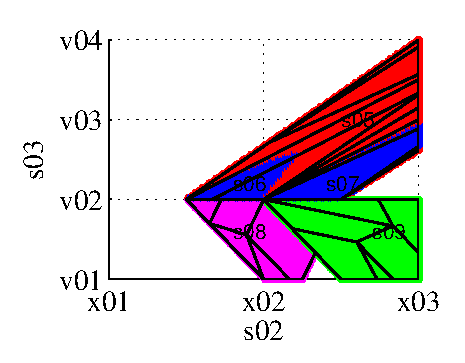
\includegraphics{ex16_1_fullreg.eps}}%
\end{psfrags}%
%
% End ex16_1_fullreg.tex
\end{document}
% See http://www.mathworks.de/matlabcentral/fileexchange/loadFile.do?objectId=4638
% for recent versions of laprint.m.
%
% created by:           LaPrint version 3.16 (13.9.2004)
% created on:           04-Mar-2010 17:41:07
% eps bounding box:     7.5 cm x 5.6116 cm
% comment:              
%
\begin{psfrags}%
\psfragscanon%
%
% text strings:
\psfrag{s02}[t][t]{\color[rgb]{0,0,0}\setlength{\tabcolsep}{0pt}\begin{tabular}{c}$x_1$\end{tabular}}%
\psfrag{s03}[b][b]{\color[rgb]{0,0,0}\setlength{\tabcolsep}{0pt}\begin{tabular}{c}$x_2$\end{tabular}}%
\psfrag{s05}[l][l]{\color[rgb]{0,0,0}\setlength{\tabcolsep}{0pt}\begin{tabular}{l}$\bf{v_1}$\end{tabular}}%
\psfrag{s06}[l][l]{\color[rgb]{0,0,0}\setlength{\tabcolsep}{0pt}\begin{tabular}{l}$\bf{v_2}$\end{tabular}}%
\psfrag{s07}[l][l]{\color[rgb]{0,0,0}\setlength{\tabcolsep}{0pt}\begin{tabular}{l}$\bf{v_2}$\end{tabular}}%
\psfrag{s08}[l][l]{\color[rgb]{0,0,0}\setlength{\tabcolsep}{0pt}\begin{tabular}{l}$\bf{v_4}$\end{tabular}}%
\psfrag{s09}[l][l]{\color[rgb]{0,0,0}\setlength{\tabcolsep}{0pt}\begin{tabular}{l}$\bf{v_3}$\end{tabular}}%
%
% xticklabels:
\psfrag{x01}[t][t]{-1}%
\psfrag{x02}[t][t]{0}%
\psfrag{x03}[t][t]{1}%
%
% yticklabels:
\psfrag{v01}[r][r]{-0.5}%
\psfrag{v02}[r][r]{0}%
\psfrag{v03}[r][r]{0.5}%
\psfrag{v04}[r][r]{1}%
%
% Figure:
\resizebox{6cm}{!}{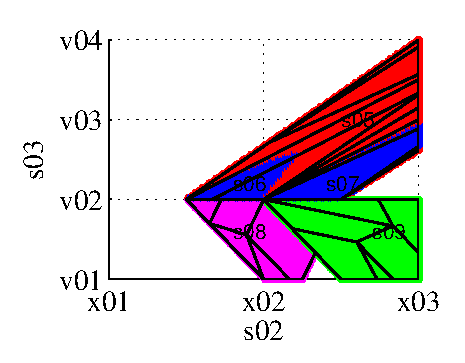
\includegraphics{ex16_1_fullreg.eps}}%
\end{psfrags}%
%
% End ex16_1_fullreg.tex
\end{document}
% See http://www.mathworks.de/matlabcentral/fileexchange/loadFile.do?objectId=4638
% for recent versions of laprint.m.
%
% created by:           LaPrint version 3.16 (13.9.2004)
% created on:           04-Mar-2010 17:41:07
% eps bounding box:     7.5 cm x 5.6116 cm
% comment:              
%
\begin{psfrags}%
\psfragscanon%
%
% text strings:
\psfrag{s02}[t][t]{\color[rgb]{0,0,0}\setlength{\tabcolsep}{0pt}\begin{tabular}{c}$x_1$\end{tabular}}%
\psfrag{s03}[b][b]{\color[rgb]{0,0,0}\setlength{\tabcolsep}{0pt}\begin{tabular}{c}$x_2$\end{tabular}}%
\psfrag{s05}[l][l]{\color[rgb]{0,0,0}\setlength{\tabcolsep}{0pt}\begin{tabular}{l}$\bf{v_1}$\end{tabular}}%
\psfrag{s06}[l][l]{\color[rgb]{0,0,0}\setlength{\tabcolsep}{0pt}\begin{tabular}{l}$\bf{v_2}$\end{tabular}}%
\psfrag{s07}[l][l]{\color[rgb]{0,0,0}\setlength{\tabcolsep}{0pt}\begin{tabular}{l}$\bf{v_2}$\end{tabular}}%
\psfrag{s08}[l][l]{\color[rgb]{0,0,0}\setlength{\tabcolsep}{0pt}\begin{tabular}{l}$\bf{v_4}$\end{tabular}}%
\psfrag{s09}[l][l]{\color[rgb]{0,0,0}\setlength{\tabcolsep}{0pt}\begin{tabular}{l}$\bf{v_3}$\end{tabular}}%
%
% xticklabels:
\psfrag{x01}[t][t]{-1}%
\psfrag{x02}[t][t]{0}%
\psfrag{x03}[t][t]{1}%
%
% yticklabels:
\psfrag{v01}[r][r]{-0.5}%
\psfrag{v02}[r][r]{0}%
\psfrag{v03}[r][r]{0.5}%
\psfrag{v04}[r][r]{1}%
%
% Figure:
\resizebox{6cm}{!}{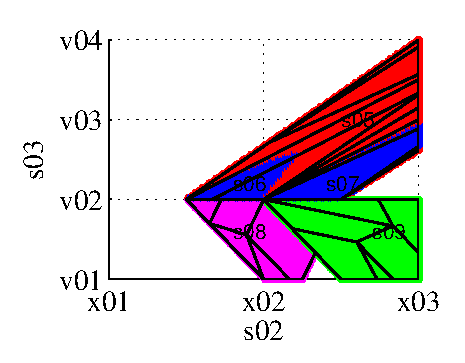
\includegraphics{ex16_1_fullreg.eps}}%
\end{psfrags}%
%
% End ex16_1_fullreg.tex
\end{document}
% See http://www.mathworks.de/matlabcentral/fileexchange/loadFile.do?objectId=4638
% for recent versions of laprint.m.
%
% created by:           LaPrint version 3.16 (13.9.2004)
% created on:           04-Mar-2010 17:41:07
% eps bounding box:     7.5 cm x 5.6116 cm
% comment:              
%
\begin{psfrags}%
\psfragscanon%
%
% text strings:
\psfrag{s02}[t][t]{\color[rgb]{0,0,0}\setlength{\tabcolsep}{0pt}\begin{tabular}{c}$x_1$\end{tabular}}%
\psfrag{s03}[b][b]{\color[rgb]{0,0,0}\setlength{\tabcolsep}{0pt}\begin{tabular}{c}$x_2$\end{tabular}}%
\psfrag{s05}[l][l]{\color[rgb]{0,0,0}\setlength{\tabcolsep}{0pt}\begin{tabular}{l}$\bf{v_1}$\end{tabular}}%
\psfrag{s06}[l][l]{\color[rgb]{0,0,0}\setlength{\tabcolsep}{0pt}\begin{tabular}{l}$\bf{v_2}$\end{tabular}}%
\psfrag{s07}[l][l]{\color[rgb]{0,0,0}\setlength{\tabcolsep}{0pt}\begin{tabular}{l}$\bf{v_2}$\end{tabular}}%
\psfrag{s08}[l][l]{\color[rgb]{0,0,0}\setlength{\tabcolsep}{0pt}\begin{tabular}{l}$\bf{v_4}$\end{tabular}}%
\psfrag{s09}[l][l]{\color[rgb]{0,0,0}\setlength{\tabcolsep}{0pt}\begin{tabular}{l}$\bf{v_3}$\end{tabular}}%
%
% xticklabels:
\psfrag{x01}[t][t]{-1}%
\psfrag{x02}[t][t]{0}%
\psfrag{x03}[t][t]{1}%
%
% yticklabels:
\psfrag{v01}[r][r]{-0.5}%
\psfrag{v02}[r][r]{0}%
\psfrag{v03}[r][r]{0.5}%
\psfrag{v04}[r][r]{1}%
%
% Figure:
\resizebox{6cm}{!}{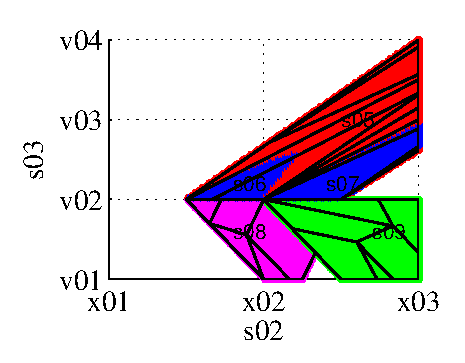
\includegraphics{ex16_1_fullreg.eps}}%
\end{psfrags}%
%
% End ex16_1_fullreg.tex
